\documentclass{beamer}

% Copyright 2010 Drow Ltd.
% 
% In principle, this file can be redistributed and/or modified under
% the terms of the GNU Public License, version 2.
% 
% However, this file is supposed to be a template to be modified
% for your own needs. For this reason, if you use this file as a
% template and not specifically distribute it as part of a another
% package/program, I grant the extra permission to freely copy and
% modify this file as you see fit and even to delete this copyright
% notice. 
\mode<presentation>
{
  \usetheme[titleline=true,
  alternativetitlepage=true,
  titlepagelogo=images/Java_logo]{Torino}
  \usecolortheme{nouvelle}
  \beamertemplatenavigationsymbolsempty
}

\usepackage{times}
\usepackage[utf8]{inputenc}
\usepackage[english,bulgarian]{babel}
\usepackage[T2A]{fontenc}

\usepackage{listings}
\lstset{language=Java,
  captionpos=b,
  tabsize=4,
  keywordstyle=\color{blue},
  commentstyle=\color{gray},
  stringstyle=\color{green},
  numbers=left,
  breaklines=true,
  showstringspaces=false,
  basicstyle=\ttfamily,
  emph={label},
  frame=shadowbox, 
  rulesepcolor=\color{blue},
  columns=fixed}

\title{Въведение в средата за програмиране Java}

\subtitle{Преглед на историята и възможностите на Java. Представяне на
  популярни среди за разработка и просто приложения.}

\author{инж. Божидар Бацов}

\institute{Drow Ltd.}

\date{26.10.2010}

\subject{Talks}
% This is only inserted into the PDF information catalog. Can be left
% out. 

% Delete this, if you do not want the table of contents to pop up at
% the beginning of each subsection:
\AtBeginSubsection[]
{
  \begin{frame}<beamer>{Съдържание}
    \tableofcontents[currentsection,currentsubsection]
  \end{frame}
}

% If you wish to uncover everything in a step-wise fashion, uncomment
% the following command: 

% \beamerdefaultoverlayspecification{<+->}


\begin{document}

\begin{frame}
  \titlepage
\end{frame}

\begin{frame}{Съдържание}
  \tableofcontents
  % You might wish to add the option [pausesections]
\end{frame}


% Since this a solution template for a generic talk, very little can
% be said about how it should be structured. However, the talk length
% of between 15min and 45min and the theme suggest that you stick to
% the following rules:  

% - Exactly two or three sections (other than the summary).
% - At *most* three subsections per section.
% - Talk about 30s to 2min per frame. So there should be between about
% 15 and 30 frames, all told.

\section{Средата за програмиране Java}

\subsection[Кои сме ние?]{Кои сме ние?}

\begin{frame}{Екип}
  \begin{itemize}
  \item
    инж. Божидар Бацов - Технически директор на Drow Ltd.
  \item
    Владимир Василев - Благ диктатор на init Lab
  \end{itemize}
\end{frame}

\begin{frame}{Комуникация}
  \begin{itemize}
  \item Пощенски списък - http://groups.google.com/group/java-in-action
  \item Ел. поща
  \item Jabber/GTalk
  \item Twitter
  \end{itemize}
\end{frame}

\begin{frame}{Формат на занятията}
  \begin{itemize}
  \item Лекции по 45 мин
  \item Почивки по 15 мин
  \item Задачки закачки за домашна работа
  \item Допълнителни практически занятия
  \item Работа по учебен проект
  \end{itemize}
\end{frame}

\subsection{Програмирането преди ерата на Java}

\begin{frame}{Програмирането през 1995}
  \begin{itemize}
    \item Lisp
    \item Pascal
    \item C
    \item Smalltalk
    \item C++
  \end{itemize}
\end{frame}

\begin{frame}{Водещи езици в последните 25 години}
  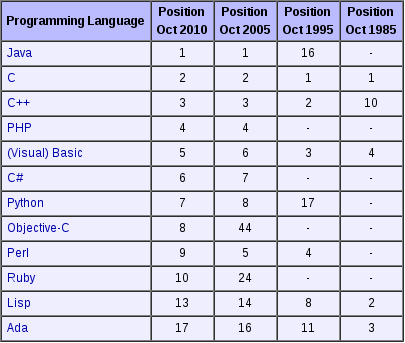
\includegraphics[width=300px,
  height=200px]{images/lang-history}
\end{frame}


\begin{frame}{Предимствата на Java}
  \begin{itemize}
  \item Простота
  \item Обектно-ориентиран
  \item Архитектурна независимост
  \item Портативност
  \item Вградена мрежова поддръжка
  \item Надеждност
  \item Сигурност
  \item Паралелизъм
  \item Динамика
  \end{itemize}
\end{frame}


\begin{frame}{Простота}
  
  \begin{itemize}
    \item Базиран на C++
    \item Изчистен синтаксис – без указатели,
    презареждане на оператори, хедър
    файлове, структури, unions и т.н.
    \item Автоматично събиране на боклука –
    \item Gargabe collection
    
  \end{itemize}
\end{frame}


\begin{frame}{Обектно ориентиран}
  \begin{itemize}
  \item Проектиран с ОО наум от самото начало
  \item Осъвършенстван ОО модел от С++
  \end{itemize}
\end{frame}


\begin{frame}{Мрежова поддръжка и паралелизъм}
  
  \begin{itemize}
    \item Мрежова поддръжка
  \begin{itemize}
  \item   Богата библиотека за работа с различни
    мрежови протоколи – TCP/IP, HTTP, FTP

  \end{itemize}
  \item Паралелизъм
    
    \begin{itemize}
    \item  Вградена поддръжка за мултипроцесори
    \item Просто и гъвкаво API за работа с нишки

    \end{itemize}

  \end{itemize}

\end{frame}


\begin{frame}{Надеждност}
  
  \begin{itemize}
    \item Липсва на указатели и асоциираните с
    тях проблеми – преливане на стека,
    достъп до невалиден указател и т.н.

    \item Няма опасност от течове на памет –
    garbage collector-а се грижи за това

  \end{itemize}

\end{frame}


\begin{frame}{Сигурност}
  
  \begin{itemize}
   \item Невъзможно е да прелее стека на
    изпълнение(runtime stack)
   \item Невъзможно е да се наруши паметта
    извън собственото адресно
    пространство
   \item Невъзможно е да се пишат/четат
    файлове без права

  \end{itemize}

\end{frame}


\begin{frame}{Преносимост}
  \begin{itemize}
  \item Стандартизирани типове – гарантирано
  е че byte е 1 байта, short е 2 байта, int –
  4, и т.н.
  \item Вградена поддръжка на различни
  файлови системи
  \end{itemize}

\end{frame}


\begin{frame}{Висока производителност}
  \begin{itemize}
  \item Производителност близка до тази на
  приложения писани на C/C++
  \item Възможност за постигане на висока
  оптимизация на бинарния код по време
  на изпълнение
\end{itemize}

\end{frame}

\begin{frame}{Раждането на Java}
  \begin{itemize}
    \item Проектът Green и James Gosling
    \item Езикът Oak
    \item Изборът на името Java
    \item Аплетите началото на Java
    \item Възходът на Java
    \item Триумфът на Java
  \end{itemize}
\end{frame}

\begin{frame}{Еволюцията на Java}
  \begin{itemize}
  \item 1996 – Java 1.0 - началото
  \item 1997 – Java 1.1 – inner classes
  \item 1998 – Java 2 1.2 – разширено API
  \item 2000 – Java 1.3 – разширено API
  \item 2004 – Java 1.4 - asserts
  \item 2004 – Java 5.0 – generics, autoboxing...
  \item 2006 – Java 6 – разширено API
  \item 2011   Java 7 invoke dynamic, project coin
  \item 2013   Java 8 closures, project jigsaw
  \end{itemize}
\end{frame}


\begin{frame}{Java и конкуренцията}
  \begin{itemize}
    \item Java срещу .NET и C\#
    \item Java срещу C/C++
    \item Java срещу JavaScript
    \item Java срещу Ruby/Python
    \item Java срещу Groovy
    \item Java срещу Scala
    \item Java срещу Clojure
  \end{itemize}
\end{frame}

\begin{frame}{Програмен език номер 1 в света.}
  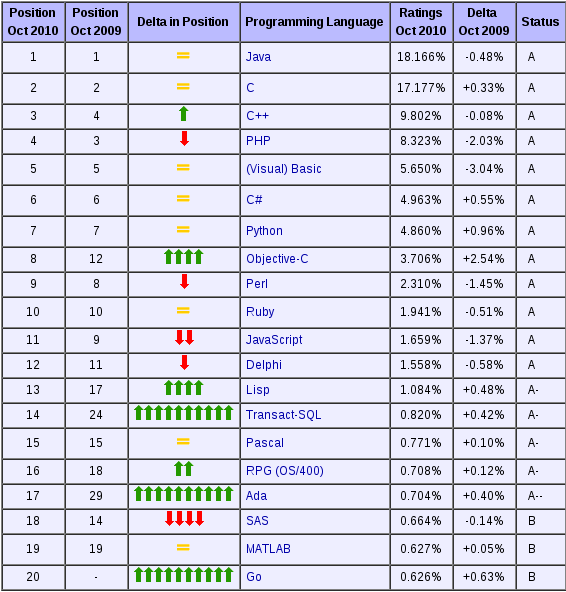
\includegraphics[width=300px,
  height=200px]{images/lang-current}
\end{frame}

\subsection{Платформата Java}

\begin{frame}{Повече от език за програмиране}

  \begin{itemize}
    \item Език за програмиране
    \item Среда за изпълнение на програми / Виртуална машина (JVM)
    \item Пакет от инструменти за разработка на приложения (Java Dev Kit)
  \end{itemize}

\end{frame}


\begin{frame}{Java платформи}
  \begin{itemize}
    \item Java Runtime Environment(JRE)
    \item Java Development Kit(JDK) SE == JRE + dev tools
    \item Java Enterprise Edition(Java EE)
    \item Java Micro Edition(Java ME)
  \end{itemize}
\end{frame}

\begin{frame}{Java имплементации}
  \begin{itemize}
  \item Различни дистрибутори – Sun, IBM,
  Oracle

  \item Референтна имплементация – Sun
  HotSpot

  \item Текуща версия – JDK 6 SE 1.6.0\_16
  \item Изтегляне от http://java.sun.com
  \end{itemize}
\end{frame}

\section{Инсталиране на Java и първи стъпки}


\begin{frame}{Инсталиране на Oracle JDK/OpenJDK}
  
  \begin{itemize}
    \item Изтегляне на подходящ дистрибутив
    \item Инсталиране под Линукс
    \item Инсталиране под Уиндоус
    \item Добавяне на изходния код и
      документацията на Java
  \end{itemize}

\end{frame}


\begin{frame}{Основни инструменти}
  
  \begin{itemize}
    \item java стартира JVM
    \item javac Java Compiler
    \item jar инструмент за работа с jar архиви
    \item javaws стартира Java Web Start
    приложение
    \item jvisualvm един не конзолен, но много
    полезен инструмент за следене статуса
    на JVM
  \end{itemize}

\end{frame}


\begin{frame}{Hey, Java!}
  
  \begin{itemize}
    \item Създаваме файл HeyJava.java
    \item Създаваме в него прост клас HeyJava
    \item Запазваме файла
    \item Компилираме – javac HeyJava.java
    \item Стартираме – java HeyJava
  \end{itemize}

\end{frame}


\begin{frame}{Интегрирани среди за разработка}
  
  \begin{itemize}
    \item Интелигентен редактор
    \item Анализ на кода
    \item Интеграция с външния системи – build
    система, issue tracker, version control
    system и т.н.
    \item Интегриран дебъгер
    \item Лесно рефакториране на кода
  \end{itemize}

\end{frame}


\begin{frame}{IntelliJ IDEA}
  \begin{itemize}
    \item www.jetbrains.com/idea
    \item Най-интелигентната среда за
    разработка на Java
    \item Изключително тежка
    \item Комерсиален и скъп продукт
    \item Лоша документация, малка общност,
    малко разширения(plugins)
  \end{itemize}
\end{frame}

\begin{frame}{Eclipse}
  \begin{itemize}
    \item www.eclipse.org
    \item Най-използваната среда за разработка
    \item Голяма общост, безброй разширения
    \item По-скоро платоформа върху, която да се
    изгражда софтуер, отколкото Java IDE
    \item Тромова система за работа с
    разширения, ниско качество на много
    разширения
  \end{itemize}
\end{frame}

\begin{frame}{NetBeans}
  
  \begin{itemize}
    \item www.netbeans.org
    \item “Официалната” среда за разработка на
    Java приложения
    \item Лесен за използване, голяма общност
    \item Най-добрата поддръжка на някои Sun-
    centric технологии
  \end{itemize}

\end{frame}



\begin{frame}{Demo}
  
\end{frame}


\begin{frame}{GitHub}
  
  \begin{itemize}
    \item Отворена общност за хостване на
    проекти с отворен код
    \item Предлагани услуги – source control
    management, wiki, issue tracker, mailing
    list, chat

    \item GitHub проект на курса - tbd
  \end{itemize}

\end{frame}

\begin{frame}{Упражение}
  
  \begin{itemize}
    \item Инсталирайте си JDK
    \item Конфигурирайте пътя за инпълнение
    \item Инсталирайте NetBeans IDE 6.7.1
    \item Пуснете си примерите от днешната
    лекция

  \end{itemize}

\end{frame}

\section*{Заключение}

\begin{frame}{Заключение}

  % Keep the summary *very short*.
  \begin{itemize}
  \item
    Java \alert{е много повече от език за програмиране}.
  \item
    JVM \alert{е целевата среда за изпълнение} на Java приложенията, а
    не физическата процесорна микроархитектура.
  \item
    За пълноценна работа с езикът и платформата Java човек трябва да
    се запознае с доста инструменти.
  \end{itemize}
  
  % The following outlook is optional.
  \vskip0pt plus.5fill
  \begin{itemize}
  \item
    Следващият път:
    \begin{itemize}
    \item
      Основния положения в езикът Java
    \item
      Повече примери, по-малко общи приказки
    \end{itemize}
  \end{itemize}
\end{frame}


\begin{frame}{Въпроси}
  \begin{center}\LARGEТук е момента да зададете вашите въпроси! :-)\end{center}
\end{frame}


\begin{frame}{Край}

  \begin{center}
    \LARGEБлагодаря Ви за вниманието!
  \end{center}
  
\end{frame}



\end{document}


